
Los controles remotos infrarrojos comerciales en general, se basan todos en el mismo principio de funcionamiento básico, un haz infrarrojo que se genera a partir de \textbf{LEDS} infrarrojos (\textbf{IREDS}), la frecuencia de la portadora es de alrededor de $40 \si[per-mode=symbol]{\kilo\hertz}$, ya que esta frecuencia es la mas inmune a las fuentes infrarrojas que comúnmente se encuentran en el ambiente, principalmente la luz solar, tubos de luz fluorescente, etc, esta portadora modula un código binario codificado en uno de tres esquemas de codificación, el primero, \textbf{pulse distance modulation} (modulación por distancia de pulsos), como se ve en la figura~\figref{fig:pulse_distance_modulation}, la información es contenida en la distancia entre los pulsos, siendo por ejemplo la distancia corta correspondiente a un $0$ y la larga a $1$, o viceversa.

 

\begin{figure}[H]
	\centering
	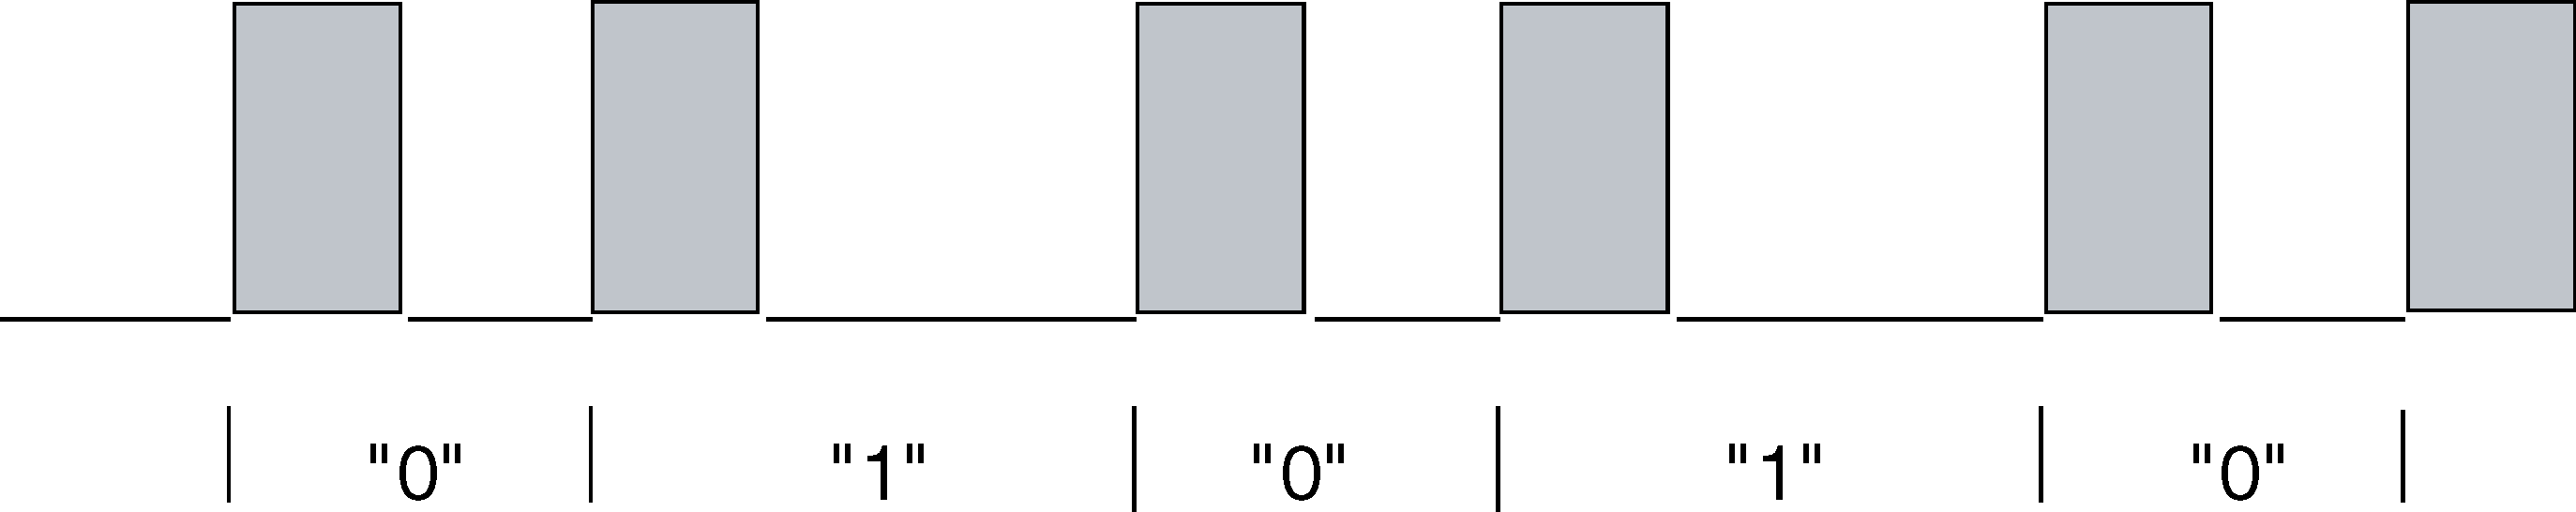
\includegraphics[width=0.95\textwidth]{img/IR/pulse_distance.png}
	\caption{\footnotesize{\textbf{pulse distance modulation}.}}
	\label{fig:pulse_distance_modulation}
\end{figure}


El segundo esquema de modulación corresponde a \textbf{pulse width modulation} (modulación por ancho de pulsos), como se ve en la figura~\figref{fig:pulse_width_modulation}, la información está codificada en el ancho de los pulsos, algo como la inversa del primer esquema.



\begin{figure}[H]
	\centering
	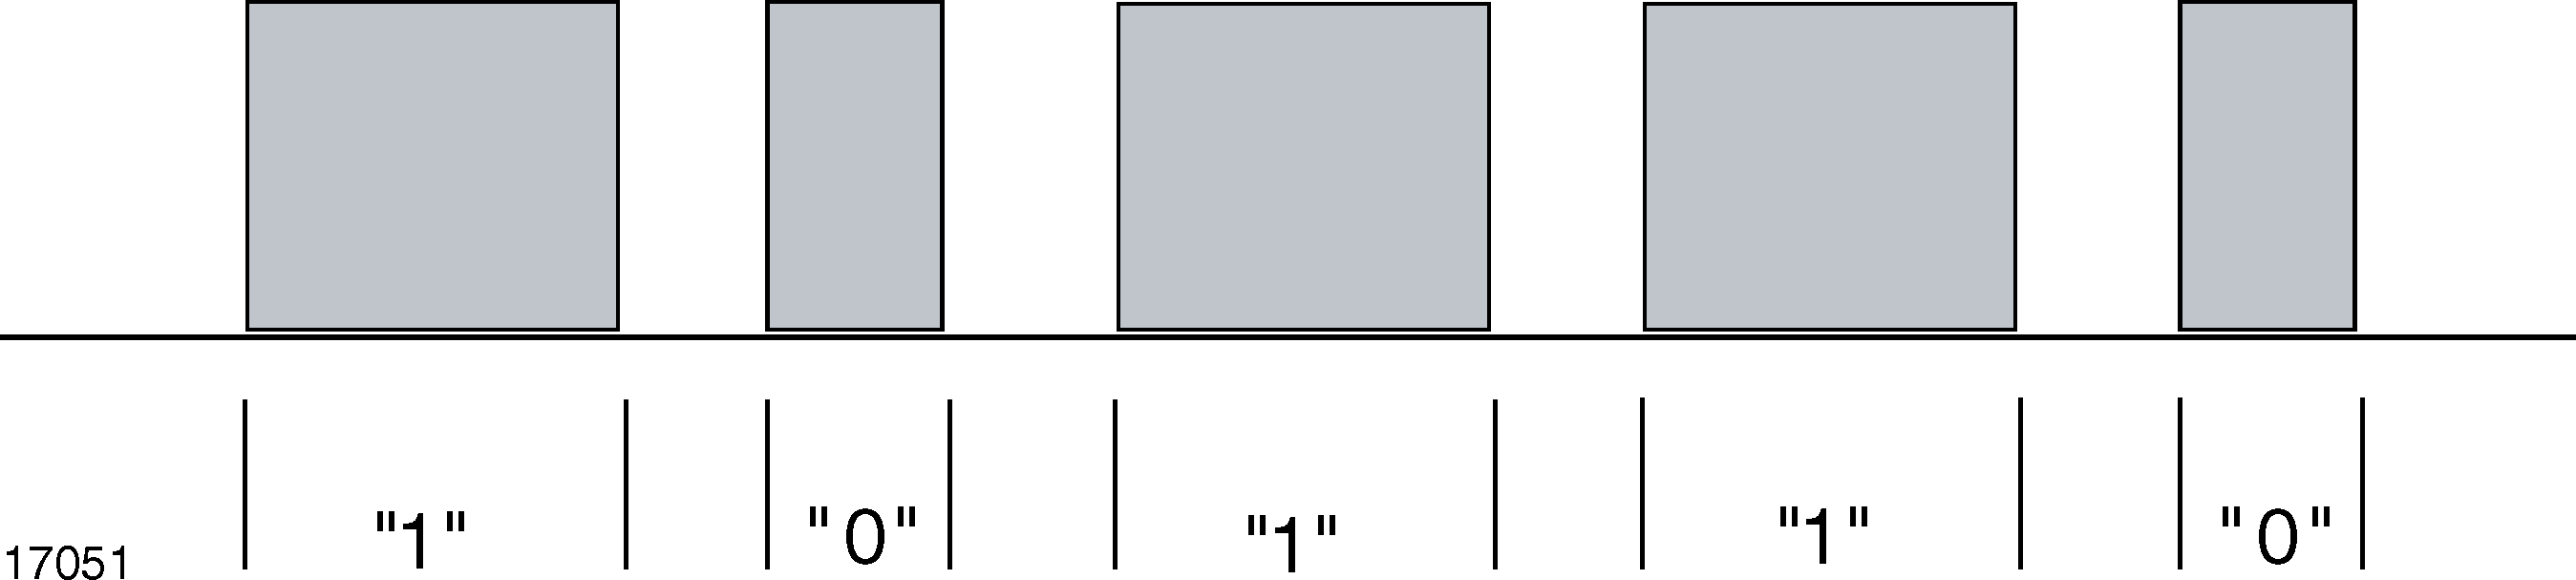
\includegraphics[width=0.95\textwidth]{img/IR/pulse_width.png}
	\caption{\footnotesize{\textbf{pulse width modulation}.}}
	\label{fig:pulse_width_modulation}
\end{figure}


El tercer y último esquema de modulación es \textbf{biphase modulation} (modulación de fase binaria), como se puede ver en la figura~\figref{fig:biphase_modulation} la información se encuentra contenida en los cambios de nivel.


\begin{figure}[H]
	\centering
	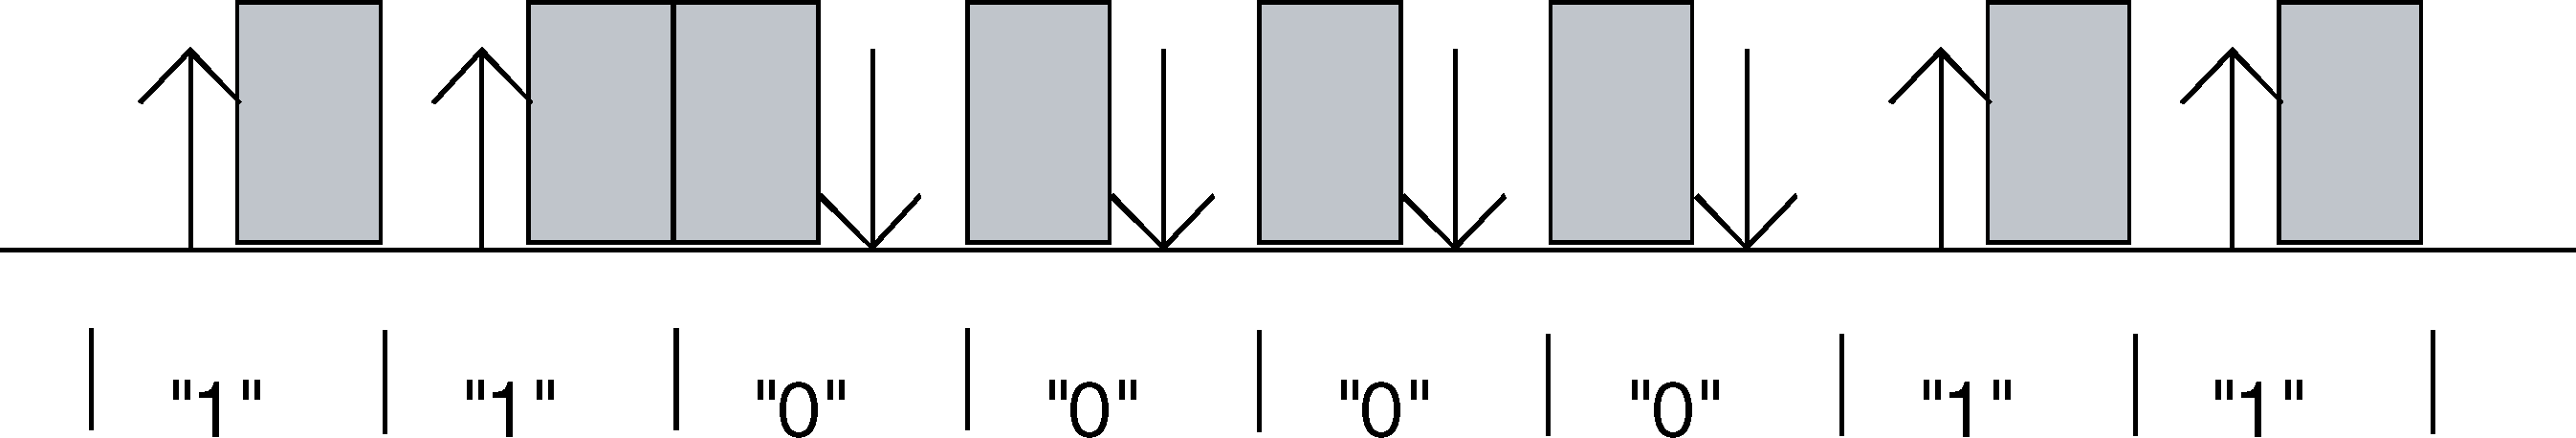
\includegraphics[width=0.95\textwidth]{img/IR/biphase.png}
	\caption{\footnotesize{\textbf{biphase modulation}.}}
	\label{fig:biphase_modulation}
\end{figure}


Estos $3$ esquemas de modulación son usados por prácticamente todas las marcas comerciales, destacándose por ejemplo el esquema \textbf{RC5} de \textbf{Philips}, figura~\figref{fig:RC5_coding}, es un esquema del tipo \textbf{biphase modulation} o el conocido esquema de codificación de \textbf{NEC} que es un esquema del tipo \textbf{pulse width modulation}, muchas otras marcas y proyectos independientes han adoptado uno de estos dos protocolos, también gran cantidad de proyectos hobbystas eligen uno de estos protocolos por su especificación pública y disponibilidad de código de decodificación de varias fuentes open source.\\

\begin{figure}[H]
	\centering
	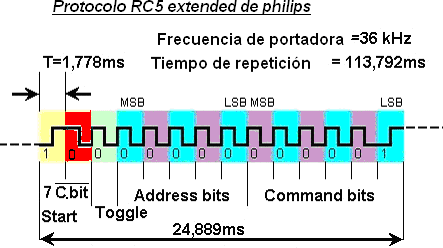
\includegraphics[width=0.95\textwidth]{img/IR/RC5_Ext.png}
	\caption{\footnotesize{código \textbf{RC5} extendido.}}
	\label{fig:RC5_coding}
\end{figure}

Todos estos protocolos utilizados a veces incluyen algunas variantes como ser, \textbf{headers} o \textbf{tails}, que se incluyen respectivamente, encabezando o terminando el código propiamente dicho que se repite mientras la tecla del control remoto se mantiene presionada, o la inclusión de un bit que cambia de una transmisión a la siguiente (usado para diferenciar una transmisión interrumpida de una diferente), pero en cualquier caso el código se encuentra modulado con la misma portadora, y algo importante, se mantiene la distancia temporal entre los bloques de código, como se puede ver por ejemplo para el caso del código \textbf{RC5} en la figura~\figref{fig:code_repetition_RC5}. En general la frecuencia de repetición del código es baja, en el orden de la decena de $\si[per-mode=symbol]{\hertz}$.


\begin{figure}[H]
	\centering
	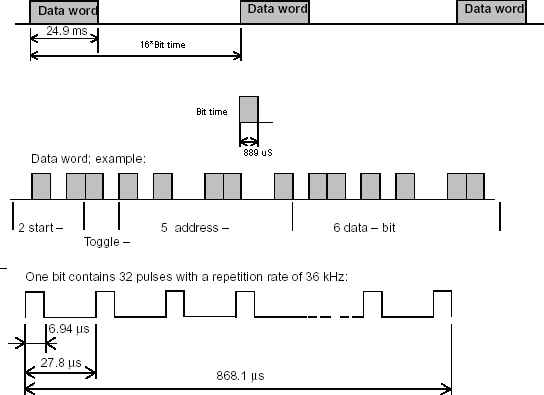
\includegraphics[width=0.95\textwidth]{img/IR/RC5_strctucture.png}
	\caption{\footnotesize{\textbf{RC5} structure.}}
	\label{fig:code_repetition_RC5}
\end{figure}


\subsubsection{Decodificación}

Como se mencionó anteriormente los controles remotos infrarrojos de uso comercial usan portadoras cercanas a $40 \si[per-mode=symbol]{\kilo\hertz}$, la demodulación necesaria previa a la decodificación que se requiere es la parte mas compleja de la recepción, ya que requiere además de detectar la señal infrarroja (comúnmente realizado con un \textbf{foto-diodo infrarrojo}), de amplificación sintonizada, control automático de ganancia, adecuación de la señal, algún tipo de \textbf{schmitt trigger} para llevar la señal a valores lógicos, etc, este esquema es tan general que ya fue integrado, de manera que incluso equipamiento comercial, utiliza estos módulos y no circuitos discretos, un ejemplo de estos módulos que se consigue en el mercado local, y que se usó en el proyecto, son los de la familia \textbf{IRM86XX}, figura~\figref{fig:IR_Module}, donde los dos últimos dígitos identifican la frecuencia central de recepción a la cual está sintonizado ese particular receptor, por ejemplo el \textbf{IRM8601} está sintonizado en $36 \si[per-mode=symbol]{\kilo\hertz}$.


\begin{figure}[H]
	\centering
	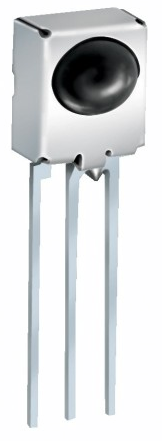
\includegraphics[width=0.15\textwidth]{img/IR/IRM86XX.png}
	\caption{\footnotesize{Módulo receptor IR.}}
	\label{fig:IR_Module}
\end{figure}



El la figura~\figref{fig:IR_Module_sch} se muestra un esquema en bloques de uno de estos módulos, donde se identifican los bloques anteriormente descriptos para la recepción y demodulación de una señal infrarroja.


\begin{figure}[H]
	\centering
	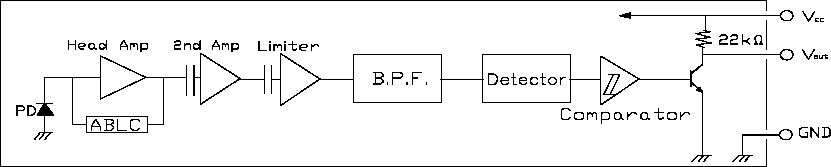
\includegraphics[width=0.95\textwidth]{img/IR/IR_module_blocks.png}
	\caption{\footnotesize{Esquema en bloques del circuito de un módulo receptor IR.}}
	\label{fig:IR_Module_sch}
\end{figure}


En general aunque cada protocolo tiene una frecuencia de portadora específica, la cercanía de las mismas hace que no sea necesario usar un módulo que coincida en forma exacta con la portadora a recibir, solo se tendrá una mayor atenuación al alejarse un poco de la frecuencia central, pero dada la gran sensibilidad de estos módulos, es común tener distancias de recepción en el orden de los $15 \si[per-mode=symbol]{\meter}$, es poco lo que afecta, y de ser necesario para un receptor mas universal podrían utilizarse un conjunto de estos módulos.



\subsection{Esquema general de transmisión y recepción}

El la figura~\figref{fig:IR_trans_rec} puede verse el esquema general de una transmisión y recepción infrarroja, en el mismo puede verse que con el módulo receptor se recupera el código ya sin modulación por la portadora, lista para ser decodificada, es esta señal la que este proyecto utiliza.


\clearpage


\begin{figure}[H]
	\centering
	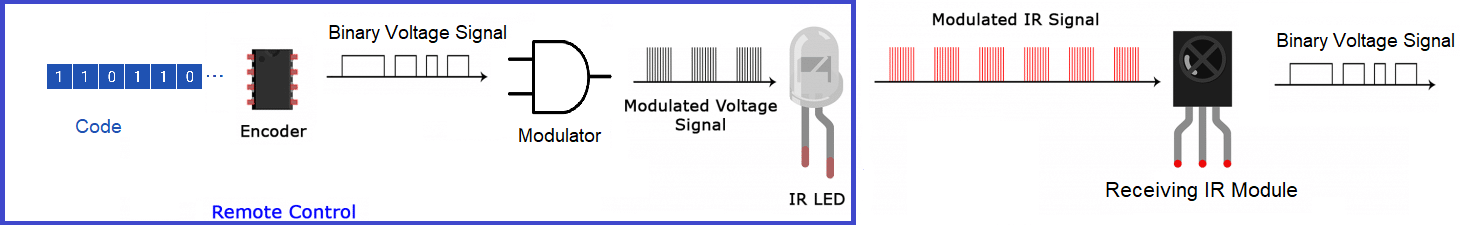
\includegraphics[width=0.85\paperwidth, angle=90]{img/IR/IR-Remote-Receiver-Modulation.png}
	\caption{\footnotesize{Esquema de transmisión y recepción IR.}}
	\label{fig:IR_trans_rec}
\end{figure}


\clearpage


La idea del circuito es bastante simple, básicamente se aprovecha la señal que genera el módulo infrarrojo para transportar el código recibido para poder volver a transmitirlo, en este caso la transmisión se realiza en banda base (no hay portadora), ya que dada la baja frecuencia de la señal, la misma puede ser transportada si gran degradación simplemente  por un cable, pero el concepto se podría ampliar para transportar la señal por radio, un enlace dedicado, \textbf{bluetooth}, \textbf{zigbee} o algo de mayor alcance como ser \textbf{LoRa}. \\

En el presente proyecto se utilizó un cable que puede ser sin problemas de hasta $30 \si[per-mode=symbol]{\meter}$ de largo y posiblemente de mayor largo, se aprovechó también el cable para transportar alimentación para la parte transmisora del circuito.


